\documentclass[border=12pt]{standalone}
\usepackage{tikz}
\usetikzlibrary{shapes.geometric, arrows.meta, positioning, calc, fit, backgrounds}
\usepackage{fontspec}
\setmainfont{DejaVu Sans}

\begin{document}
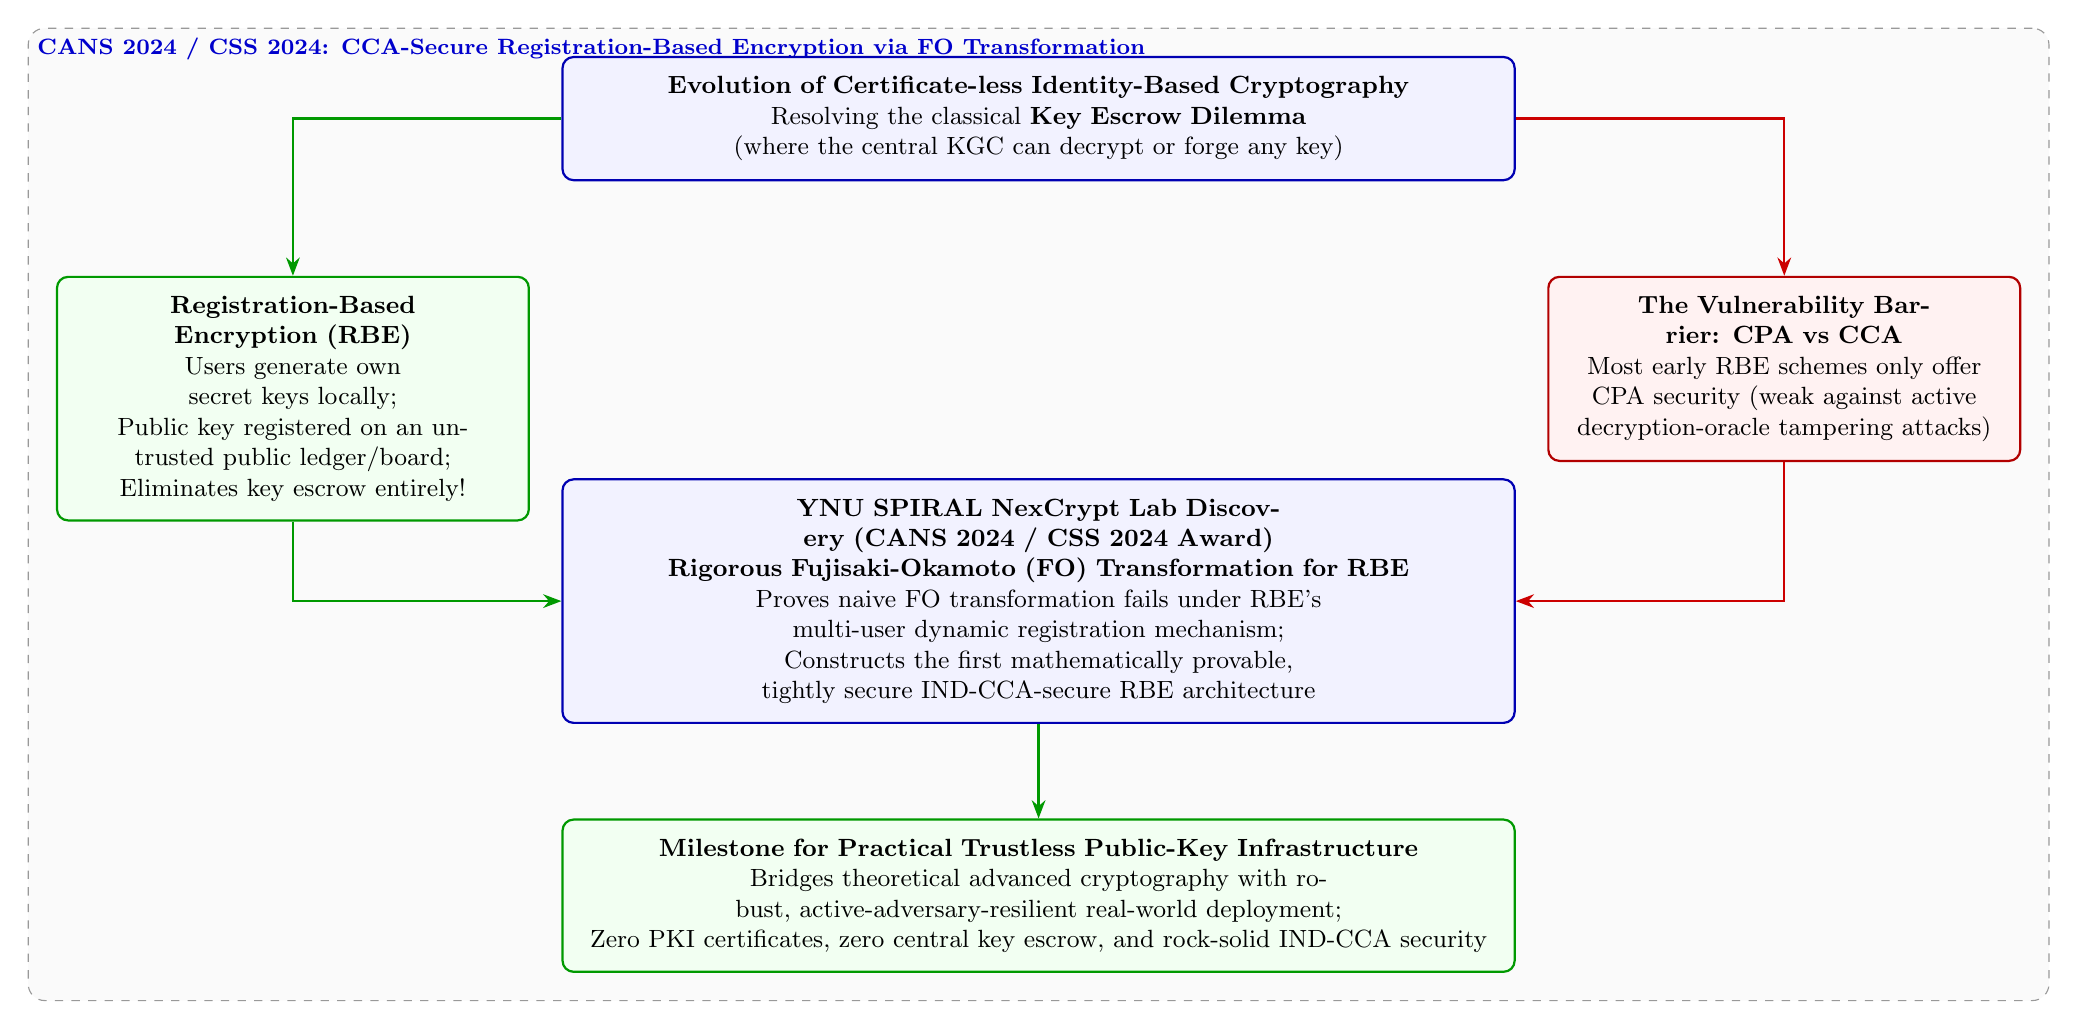
\begin{tikzpicture}[
    font=\small,
    >=Stealth,
    node distance=1.2cm,
    block/.style={rectangle, draw=blue!70!black, fill=blue!5, rounded corners=4pt, thick, align=center, inner sep=7pt},
    alertblock/.style={rectangle, draw=red!70!black, fill=red!5, rounded corners=4pt, thick, align=center, inner sep=7pt},
    greenblock/.style={rectangle, draw=green!60!black, fill=green!5, rounded corners=4pt, thick, align=center, inner sep=7pt},
    amberblock/.style={rectangle, draw=orange!80!black, fill=orange!5, rounded corners=4pt, thick, align=center, inner sep=7pt},
    groupbox/.style={draw=black!40, dashed, rounded corners=6pt, fill=black!2, inner sep=10pt}
]

    % Top: Overcoming Identity-Based Encryption (IBE) Limits
    \node[block, text width=11.6cm] (ibe) {\textbf{Evolution of Certificate-less Identity-Based Cryptography}\\Resolving the classical \textbf{Key Escrow Dilemma} (where the central KGC can decrypt or forge any key)};

    % Left: Registration-Based Encryption (RBE) Concept
    \node[greenblock, below left=1.2cm and 0.4cm of ibe, text width=5.5cm] (rbe) {\textbf{Registration-Based Encryption (RBE)}\\Users generate own secret keys locally;\\Public key registered on an untrusted public ledger/board;\\Eliminates key escrow entirely!};

    % Right: The Real-World Barrier: CCA Security
    \node[alertblock, below right=1.2cm and 0.4cm of ibe, text width=5.5cm] (cca) {\textbf{The Vulnerability Barrier: CPA vs CCA}\\Most early RBE schemes only offer CPA security (weak against active decryption-oracle tampering attacks)};

    \draw[->, thick, green!60!black] (ibe) -| (rbe);
    \draw[->, thick, red!80!black] (ibe) -| (cca);

    % Middle: YNU Breakthrough (CANS 2024 / CSS 2024 Award)
    \node[block, below=1.2cm of $(rbe)!0.5!(cca)$, text width=11.6cm] (breakthrough) {\textbf{YNU SPIRAL NexCrypt Lab Discovery (CANS 2024 / CSS 2024 Award)}\\\textbf{Rigorous Fujisaki-Okamoto (FO) Transformation for RBE}\\Proves naive FO transformation fails under RBE's multi-user dynamic registration mechanism;\\Constructs the first mathematically provable, tightly secure IND-CCA-secure RBE architecture};

    \draw[->, thick, green!60!black] (rbe) |- (breakthrough);
    \draw[->, thick, red!80!black] (cca) |- (breakthrough);

    % Bottom: Future Communication Impact
    \node[greenblock, below=1.2cm of breakthrough, text width=11.6cm] (impact) {\textbf{Milestone for Practical Trustless Public-Key Infrastructure}\\Bridges theoretical advanced cryptography with robust, active-adversary-resilient real-world deployment;\\Zero PKI certificates, zero central key escrow, and rock-solid IND-CCA security};

    \draw[->, thick, green!60!black] (breakthrough) -- (impact);

    \begin{scope}[on background layer]
        \node[groupbox, fit=(ibe) (rbe) (cca) (breakthrough) (impact), label={[anchor=north west, font=\footnotesize\bfseries, blue!80!black]north west:CANS 2024 / CSS 2024: CCA-Secure Registration-Based Encryption via FO Transformation}] {};
    \end{scope}

\end{tikzpicture}
\end{document}
